\documentclass[12pt,a4paper]{article}
\usepackage[utf8]{inputenc}
\usepackage[T1]{fontenc}
\usepackage{amsmath}
\usepackage{amsfonts}
\usepackage[francais]{babel}
\usepackage{amssymb}
\usepackage{graphicx}
\usepackage[top=2.00cm]{geometry}
\usepackage{enumitem}
%\usepackage{tikz}
\usepackage{mathtools}
%\usepackage{pgfplots}
%\usetikzlibrary{plotmarks}
\usepackage{bigcenter}
\usepackage{multicol}
\usepackage{minibox}

%Modif des enumerates numeros en gras. leftmargin=*,
\setlist[enumerate]{label=\textbf{\arabic*}.}

\usepackage{titlesec}
%modif des titres de section diminuer la taille
\titleformat{\section}
  {\normalfont\fontsize{14}{15}\bfseries}{\thesection}{1em}{}
\titleformat{\subsection}
  {\normalfont\fontsize{12}{15}\bfseries}{\thesubsection}{1em}{}


\author{CHARNAY Valentin, FINOT Sylvain}
\title{Compte rendu de TP : \\ Modulation}
\date{6 janvier 2017}
\begin{document}

\maketitle
L'objectif de ce TP est de moduler et démoduler un signal électrique (modulation d'amplitude AM puis modulation de fréquence FM) qui modélise le principe d'émission/réception.
\section{Modulation d'amplitude}
\begin{enumerate}
\item Modulation :\\
Pour la modulation d'amplitude on utilise un montage non inverseur (AOP).
\begin{multicols}{2}
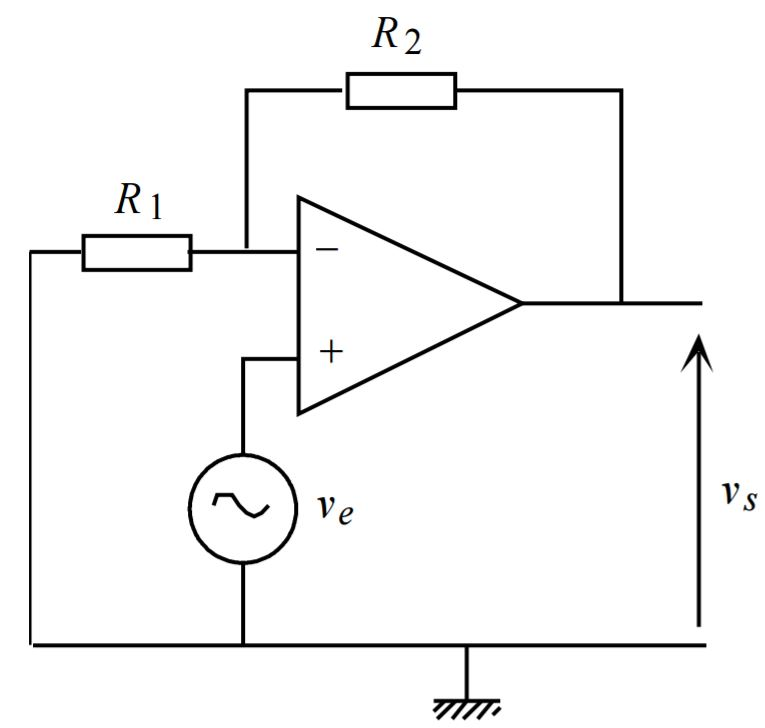
\includegraphics[scale=0.2]{MontageNonInv}
\columnbreak
\\
Le lien entre la tension d'entrée $v_e$ et de sortie $v_s$ est :
$$v_s=(1+\dfrac{R_2}{R_1})v_e$$
\end{multicols} 
Le but est maintenant d'utiliser un signal d'entrée $v_e$ ayant une fréquence relativement élevée : c'est notre onde porteuse. Nous devons ajouter l'information que nous voulons transporter à cette porteuse. Afin d'y parvenir, nous devons trouver un système nous permettant d'obtenir un gain variable en fonction de la fréquence. Ainsi, l'amplitude du signal de sorti est directement reliée à notre signal jouant le rôle d'information (onde modulante).\\
La méthode consiste a remplacer la résistance R$_1$ par un transistor à effet de champs qui se comporte comme une résistance variable (entre le drain et la source) pilotée par la tension appliquée entre la grille et la source notée $V_{GS}$ ou encore E.\\
Remarques : 
\begin{itemize}[label=\textbullet]
\item Le transistor possède une résistance propre "à vide", lorsque qu'aucune tension est appliquée entre la grille et la source ($E=0$).
\item Pour que le transistor ait ce comportement il faut : $E<0$
\item Il existe une tension $V_p$ dite de pincement pour laquelle la résistance du transistor devient quasi-infinie.
\end{itemize}
\begin{multicols}{2}
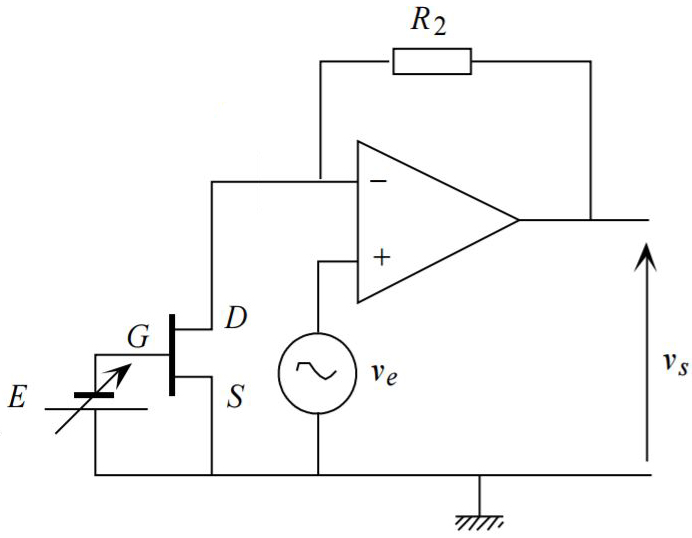
\includegraphics[scale=0.4]{MontageAmpTrans}
\columnbreak
\\
La résistance aux bornes du transistor est donnée par :
$$R_{DS}=\dfrac{R_0}{1-\dfrac{V_{GS}}{V_P}}$$

\begin{align*}
\dfrac{v_s}{v_e}&=1+\dfrac {R_{2}} {R_{0}}( 1-\dfrac {v_{GS}} {v_{p}})\\
&=( 1+\dfrac {R_{2}} {R_{0}}) -\dfrac {v_{GS}R_{2}} {v_{p}R_{0}}
\end{align*}

\end{multicols}
Nous avons vu dans le premier TP sur les AOP que le produit gain-bande d'un AOP était une constante propre au composant. La porteuse étant a une fréquence assez élevée($\approx 10^5Hz$), il faut choisir un AOP avec un bon produit gain-bande. On fixera aussi l'ordre de grandeur du gain à environ 2 en jouant sur R$_2$.\\
D'après l'expression obtenue, le gain maximal est obtenu pour E=0. Il vaut alors : $\dfrac{v_s}{v_e}=1+\dfrac {R_{2}} {R_{0}}$\\
Nous avons pris R$_2$=560$\Omega$, le gain maximal (mesuré) est alors de 2,4. En faisant varier E, le comportement est linéaire pour $0>E>-1$\\
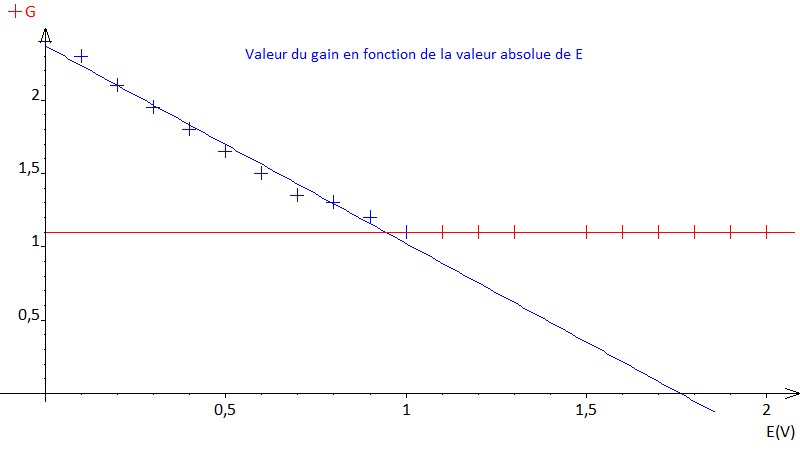
\includegraphics[scale=0.5]{Gain.jpg}
En faisant varier l'amplitude de la porteuse, on remarque que si celle ci est trop grande le signal est déformé.\\
La dernière étape consiste à remplacer E qui était fixe et continue jusqu'à présent par notre modulante tout en tenant compte des contraintes imposées par le transistor. Il faut donc veiller a avoir une modulante de faible amplitude pour que le gain soit bien linéaire et constamment négative pour ne pas détériorer le transistor. On règle au préalable le générateur basse fréquence (=modulante) en amplitude et en ajoutant un Offset continue au signal.\\
Par mesure de précautions nous ajouterons une résistance et une diode de redressement qui viendra court circuiter le transistor si le signal devient positif. La résistance sert juste a limiter le courant passant dans la diode pour ne pas la griller.\\
En regardant la sortie sur l'oscilloscope, on voit bien que celle si est conforme a l'entrée.\\
Ci dessous différents signaux (courbes) et leur sortie obtenue (enveloppes)
\begin{bigcenter}
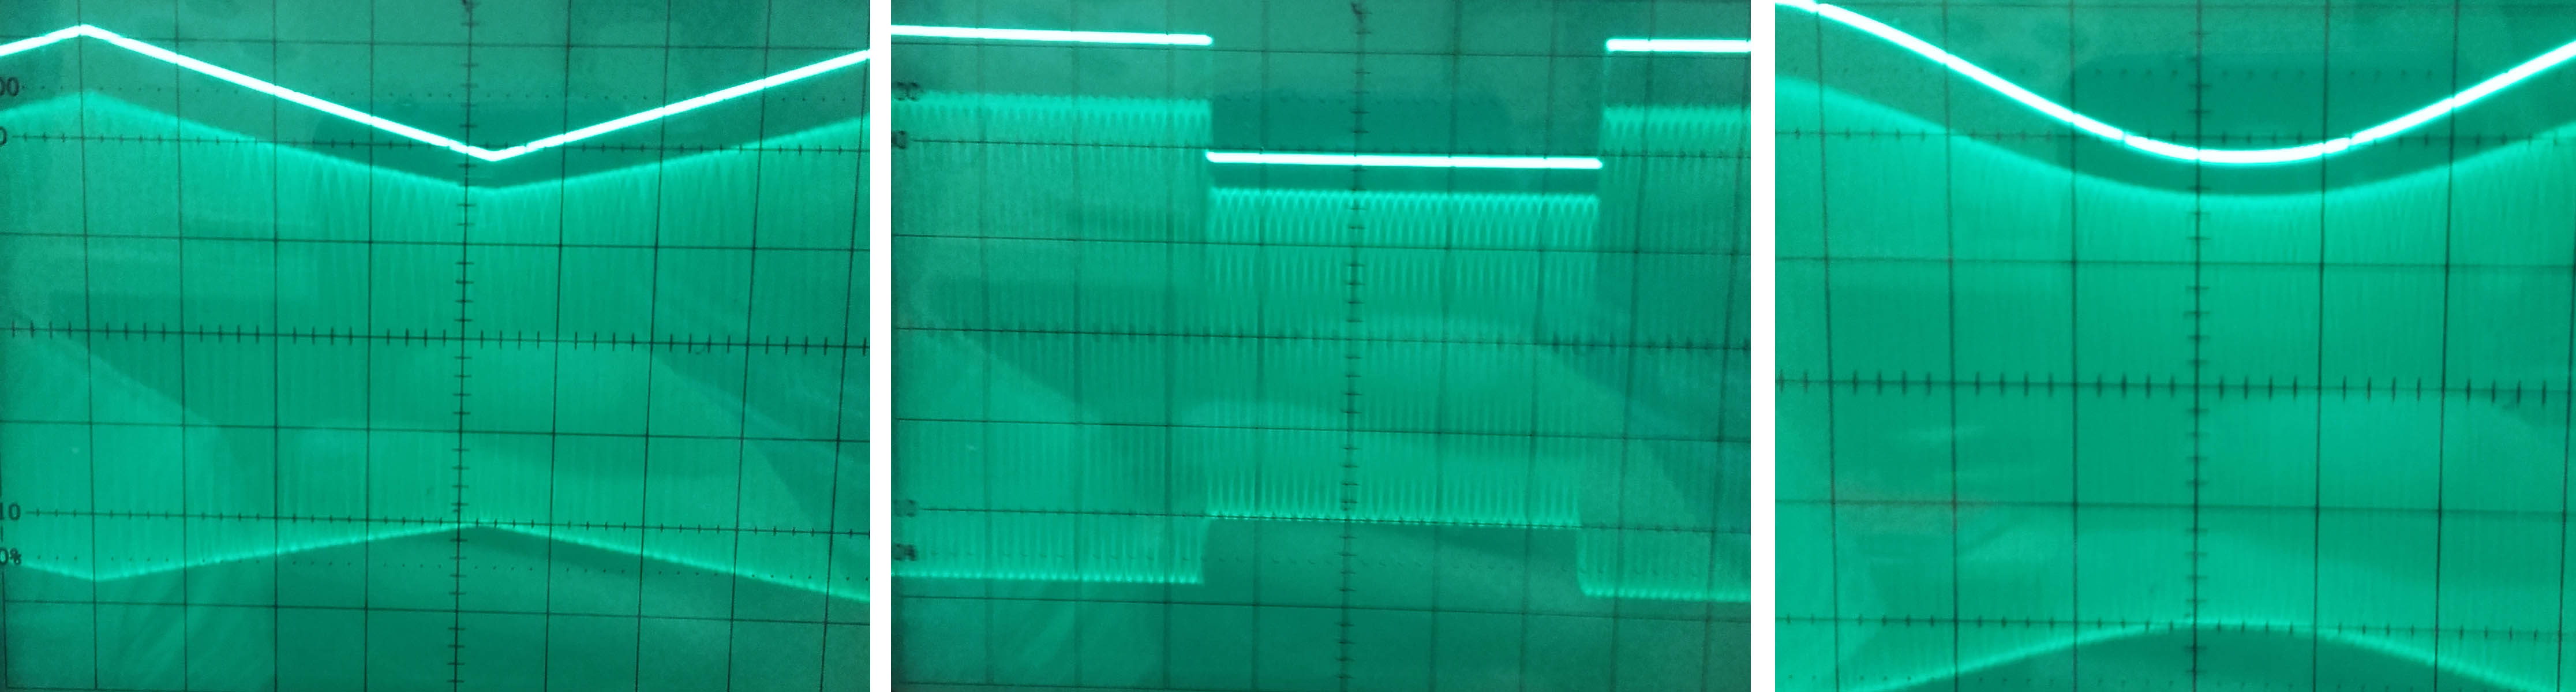
\includegraphics[scale=0.1]{ModAmp}
\end{bigcenter} 
Ces résultats ont été obtenus avec une modulante de 440Hz et une porteuse de 200kHz.\\
Remarque : l'oscilloscope déclenche sur un seul canal (ici l'entrée), c'est pour cette raison que la sortie apparait comme un bloc, les oscillations sont beaucoup plus rapides que la fréquence de balayage et donc bougent pendant un balayage. Une solution pour y remédier, le rapport entre la fréquence de la porteuse et de la modulante doit être un entier. De cette manière même si la sortie oscille, pendant un balayage elle revient au même état.
\item Démodulation :\\
\\
\includegraphics*[scale=1]{DDC}
Ici en rouge le signal, en noir la tension aux bornes du condensateur.
Pour démoduler le signal, on utilise un détecteur de crête constitué d'une diode de détection laissant passé que les courants positif et d'un dipôle RC.
On cherche un temps caractéristique $\tau = R.C$ tel que la chute de modulation soit analysé $t=\frac{2\pi}{\Omega}>> \tau$ mais pour bien lire la monté il nous faut $\tau << T = \frac{2\pi}{\omega}$. On doit donc trouver R et C tel que : 

\begin{align*}
\frac{2\pi}{\omega}&>> R.C >>  \frac{2\pi}{\Omega}\\
\iff \frac{1}{440,8}&>> R.C >>  \frac{1}{200,3.10^3}\\
\approx 2,3.10^{-3}&>>R.C>>5.10^{-6}
\end{align*}
Pour choisir $\tau$, nous avons calculer $x$ tel que :
\begin{align*}
\frac{2\pi}{\omega}.\frac{1}{x}&=\frac{2\pi}{\Omega}.x=\tau\\
\iff \dfrac{1}{f}.\frac{1}{x} &=\frac{1}{F}.x\\
\implies x&=\sqrt{\dfrac{F}{f}}\\
\tau&=\dfrac{1}{F}.\sqrt{\dfrac{F}{f}}
\end{align*} 
Avec  nos valeurs de $F(\omega) = 200$ kHz et $f(\Omega) = 440 $ Hz on estime $\tau \approx 0.1$ ms.
On choisit alors une capacité de 1 nF et une résistance de 100 k$\Omega$.\\

En réalisant le montage, nous n'avons eu aucun défaut de démodulation. Le signal était très nette et fidèle au signal d'entrée. On peut tout de même faire deux hypothèses (que nous avons retrouvé chez d'autres groupes et dans la démodulation lors de la partie modulation en fréquence).
\begin{itemize}
\item Si la constante de temps $\tau$ est trop petite, le signal peut conservé des crans à la fréquence de la porteuse. Ce n'est pas très gênant, il suffit de refiltrer le signal.
\item En revanche, si on prend une constante de temps trop grande, on risque de manquer des oscillations (en particulier les minima de la sinusoïde)
\end{itemize}
\end{enumerate}


\section{Modulation de fréquence}
Dans cette partie, on va utiliser un montage avec AOP de type Oscillateur Astable (que nous avons déjà étudié dans notre premier TP). On se rappelle alors que la période est définie par : 
$$T=2.R.C.\ln(1+2\dfrac{R_2}{R_1})$$
On veut une fréquence de quelques kHz. On fait alors l'approximation suivante : en prenant R$_1$ = R$_2$ $\implies$ $\ln(1+2\dfrac{R_2}{R_1}) = \ln 3 \approx 1$. Ainsi,
\begin{align*}
T\approx 2.R.C &\implies F = \dfrac{1}{2.RC} \quad \text{et} \quad F > 10^4 \\[0.5em]
&\iff R<\dfrac{1}{2.C.10^4} \quad \text{avec } C=2.10^{-11}F\\[1em]
&\implies R<2,5.10^6\Omega
\end{align*}
Rappel : Le calcul d'incertitudes se fait avec la formule suivante
$$\boxed{\Delta f \equiv \sqrt {\sum _{i}^{N}\left( \dfrac {\partial f} {\partial x_{i}}\right) ^{2}\cdot (\Delta x_i)^{2}}}$$
On choisit R=560k$\Omega$, R$_1$=R$_2$=1k$\Omega$. Sachant que les résistances ont une précision de 5\%, on trouve alors : \\
\begingroup
\addtolength{\jot}{0.5em}
\begin{align*}
F&=\dfrac {1} {2RC\ln \left( 1+\dfrac {2R_2} {R_1}\right) }\\
&=20,3.10^{3}Hz\\
\Delta F &= \frac{1}{2} \sqrt{\frac{4 R^2 \left(\text{$\Delta $R2}^2 \text{R1}^2+\text{$\Delta $R1}^2 \text{R2}^2\right)+\text{$\Delta $R}^2 \text{R1}^2 (\text{R1}+2 \text{R2})^2 \ln ^2\left(\frac{2 \text{R2}}{\text{R1}}+1\right)}{C^2 R^4 \text{R1}^2 (\text{R1}+2 \text{R2})^2 \ln ^4\left(\frac{2 \text{R2}}{\text{R1}}+1\right)}}\\
&=...\\
&=2677Hz
\end{align*}
\endgroup
Expérimentalement on trouve une période 40$\mu$s $\pm2\mu$s, ce qui nous donne :
\begin{align*}
F&=\dfrac{1}{T}\\
&=\dfrac{1}{40.10^{-6}}=25.10^3 Hz\\
\Delta F &= \sqrt{\frac{\text{$\Delta $T}^2}{T^4}}\\
&=\sqrt{\frac{\left(2.10^{-6}\right)^2}{\left(40.10^{-6}\right)^4}}\\
&=1250Hz
\end{align*}
La valeur expérimentale correspond bien à la valeur théorique calculée.\\
On teste ensuite en faisant varier E par de 0 à 2V et on remarque ainsi que si E augmente, la période diminue et donc la fréquence augmente. \\
\begin{center}
\begin{tabular}{l|l|l}
E   & T    & F     \\
(V) & ($\mu$s) & (kHz) \\ \hline
0   & 36   & 27,8  \\
0,5 & 35   & 28,6  \\
1   & 34   & 29,4  \\
1,5 & 33   & 30,3 
\end{tabular}
\end{center}
On remarque que la période diminue de moins en moins lorsque E augmente (Entre 5V et 10V il n'y a que 3$\mu$s d'écart). Donc on se placera avec une modulante de faible amplitude.\\
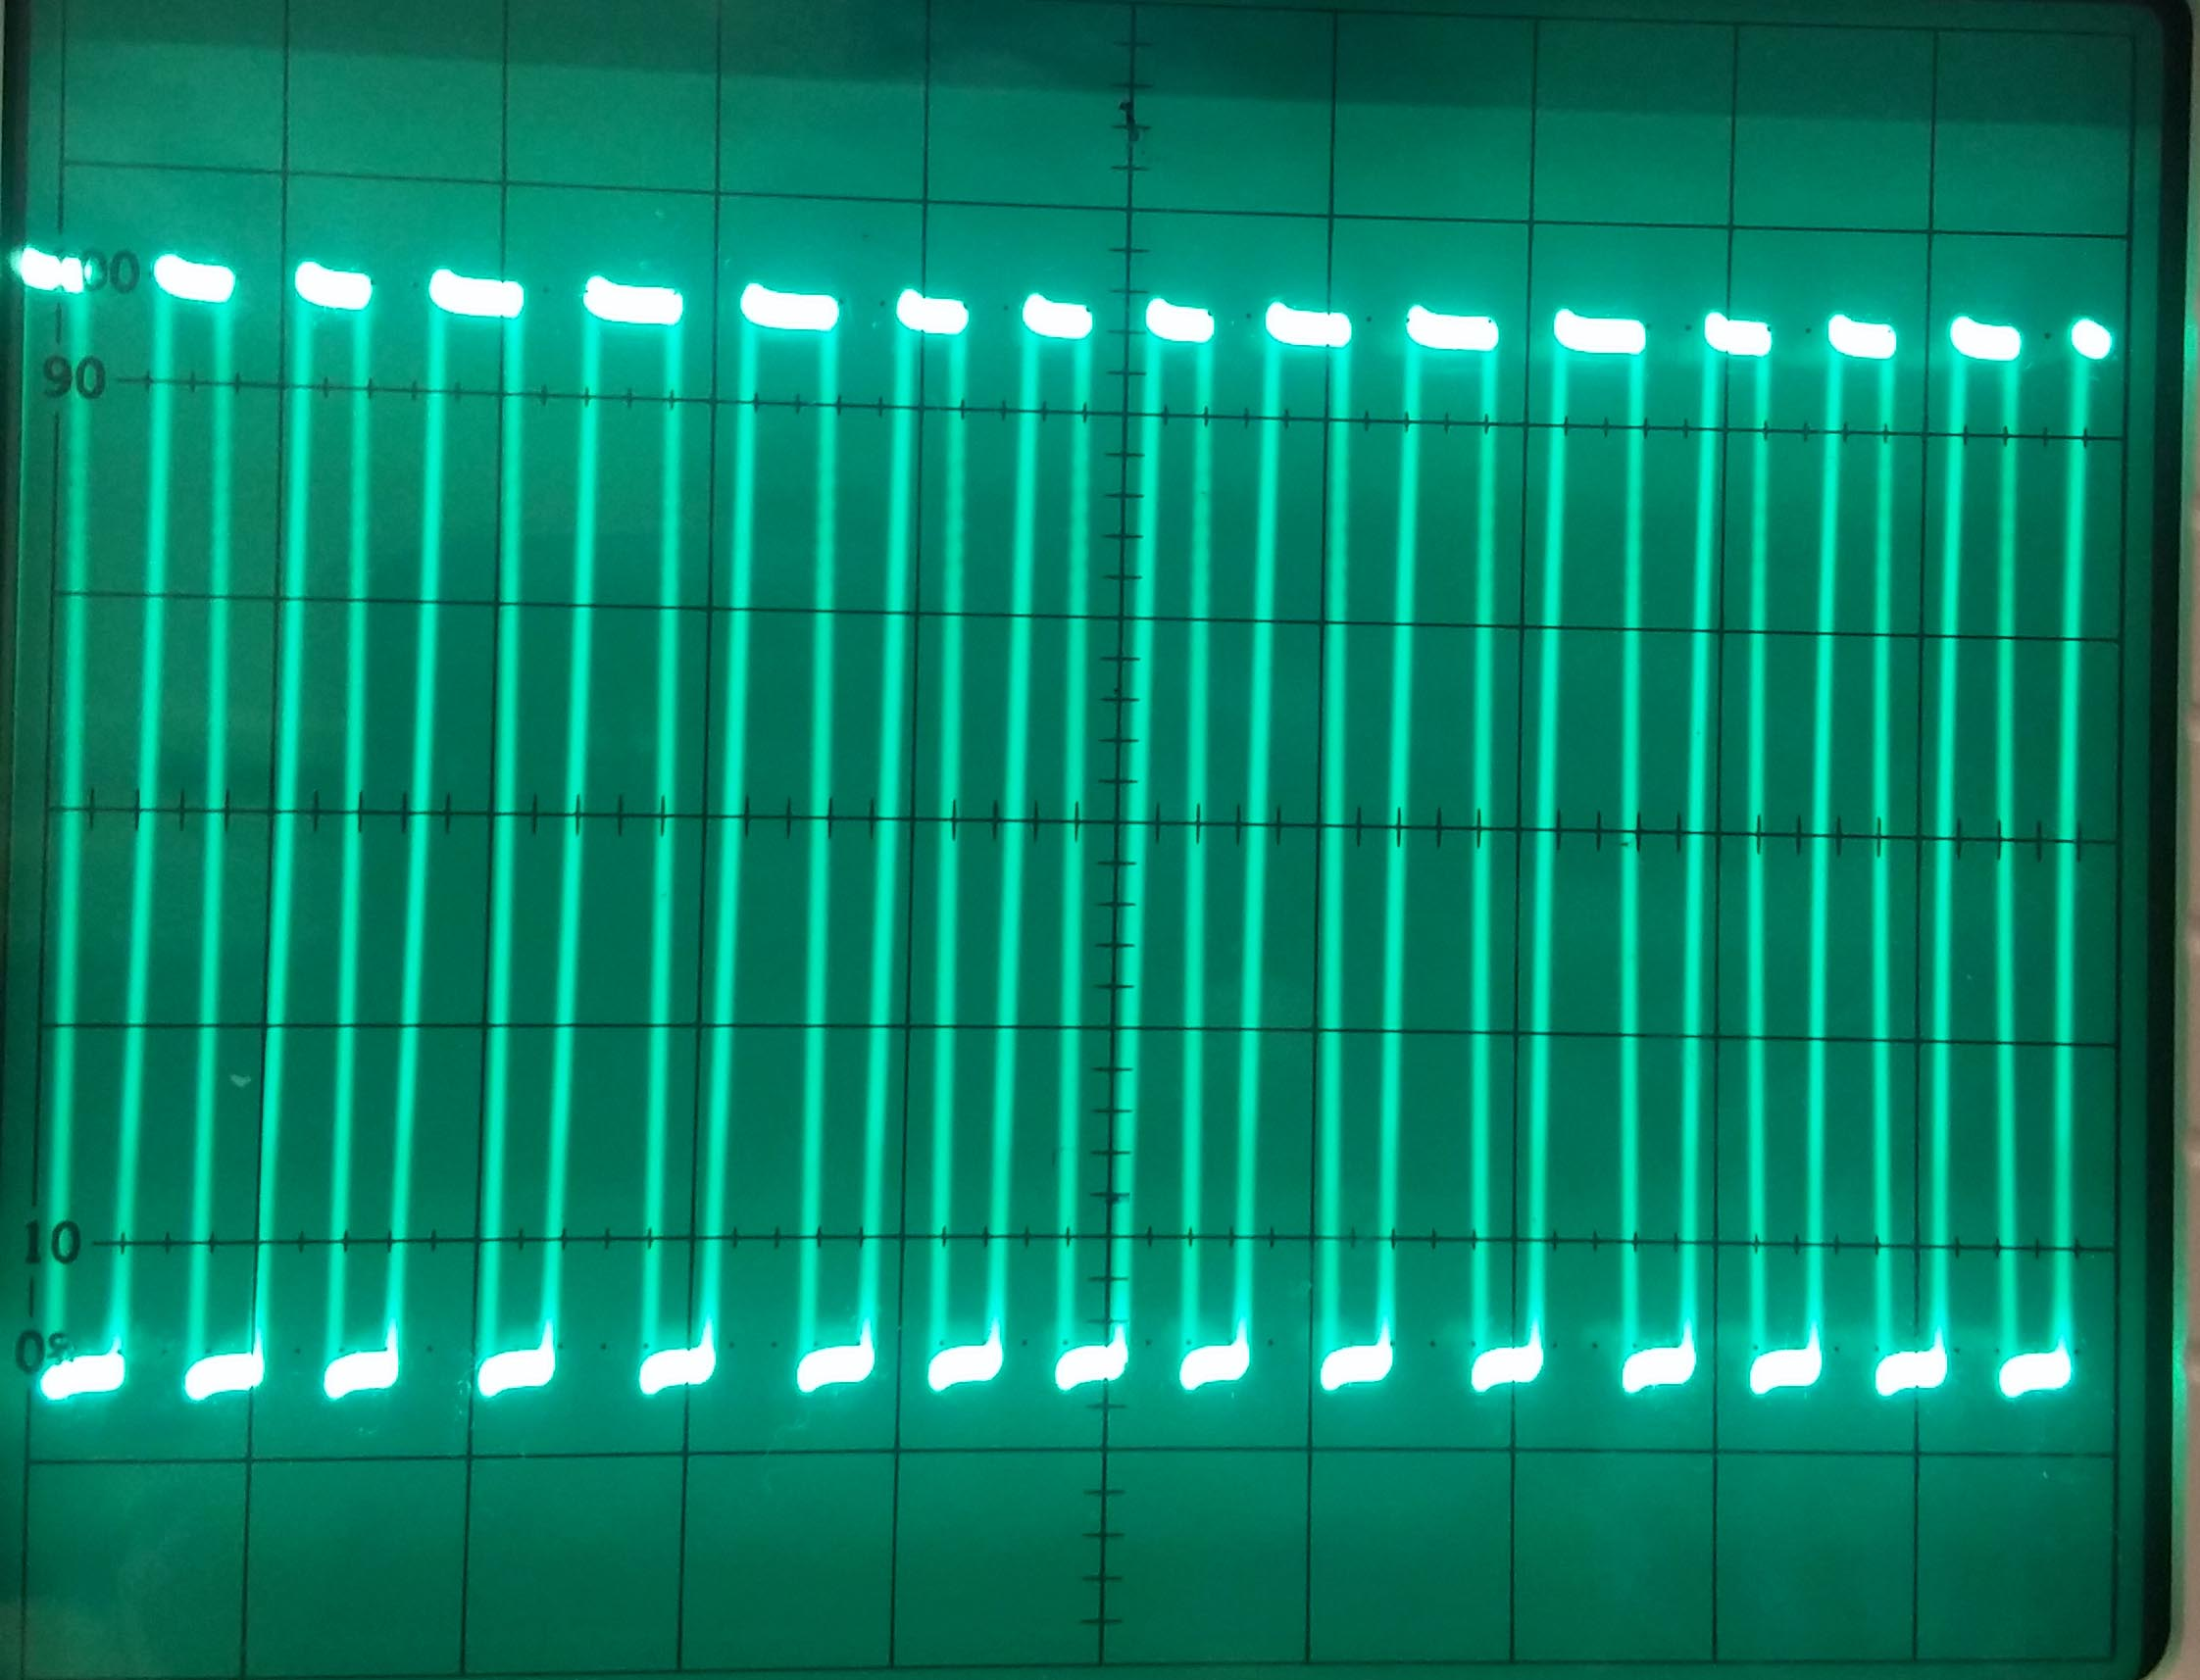
\includegraphics[scale=0.1]{modfrecre}
\\
On remarque bien la modulation en fréquence sur ces créneaux.

\section{Démodulation du signal (en fréquence)}
La méthode utilisée pour démoduler notre signal consiste à convertir notre signal modulé en fréquence en signal modulé en amplitude puis utiliser l'étage de démodulation en amplitude (détecteur de crêtes) vu précédemment. Pour effectuer cette conversion FM $\rightarrow$ AM, il nous faut un montage ayant un gain variable en fréquence et qui plus est, la variation de gain doit être relativement important pour une faible variation de fréquence.\\
L'idée est alors d'utiliser un circuit RLC comportant une résonance et se placer sur la pente (-40dB/décade?)\\
On rappelle les expressions de la pulsation propre et du facteur de qualité:
$$\omega_0=\dfrac{1}{\sqrt{L.C}}\qquad Q=\dfrac{1}{R}.\sqrt{\dfrac{L}{C}}$$
On ajuste les valeurs de R, L et C pour que la pulsation moyenne $\omega_p$ de la porteuse  soit située sur le flanc droit de la courbe de résonance (donc $\omega_0$ légèrement inférieure à $\omega_p$), et que le facteur de qualité Q du circuit soit suffisamment élevé (Q > 5) ce qui assure que la pente de cette courbe soit raide autour de $\omega_p$.
Notre hypothèse concernant le choix du flanc droit de la courbe de résonance est que la pente de celui ci est constante sur un plus grand intervalle, on limite ainsi d'éventuelles distorsions. (voir ci-dessous)\\
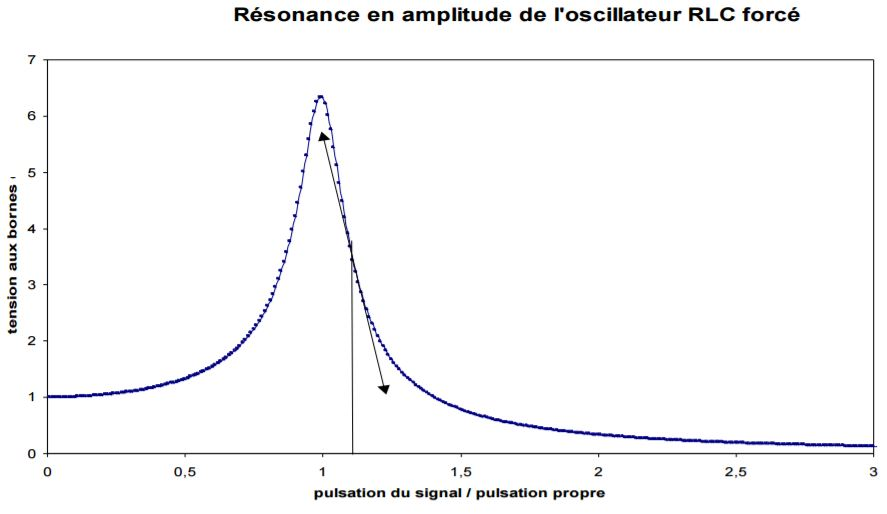
\includegraphics[scale=0.6]{courbe}\\
On propose ce circuit ou Vs notre signal modulé en fréquence et u$_c$ le signal modulé/converti en AM\\
\begin{center}
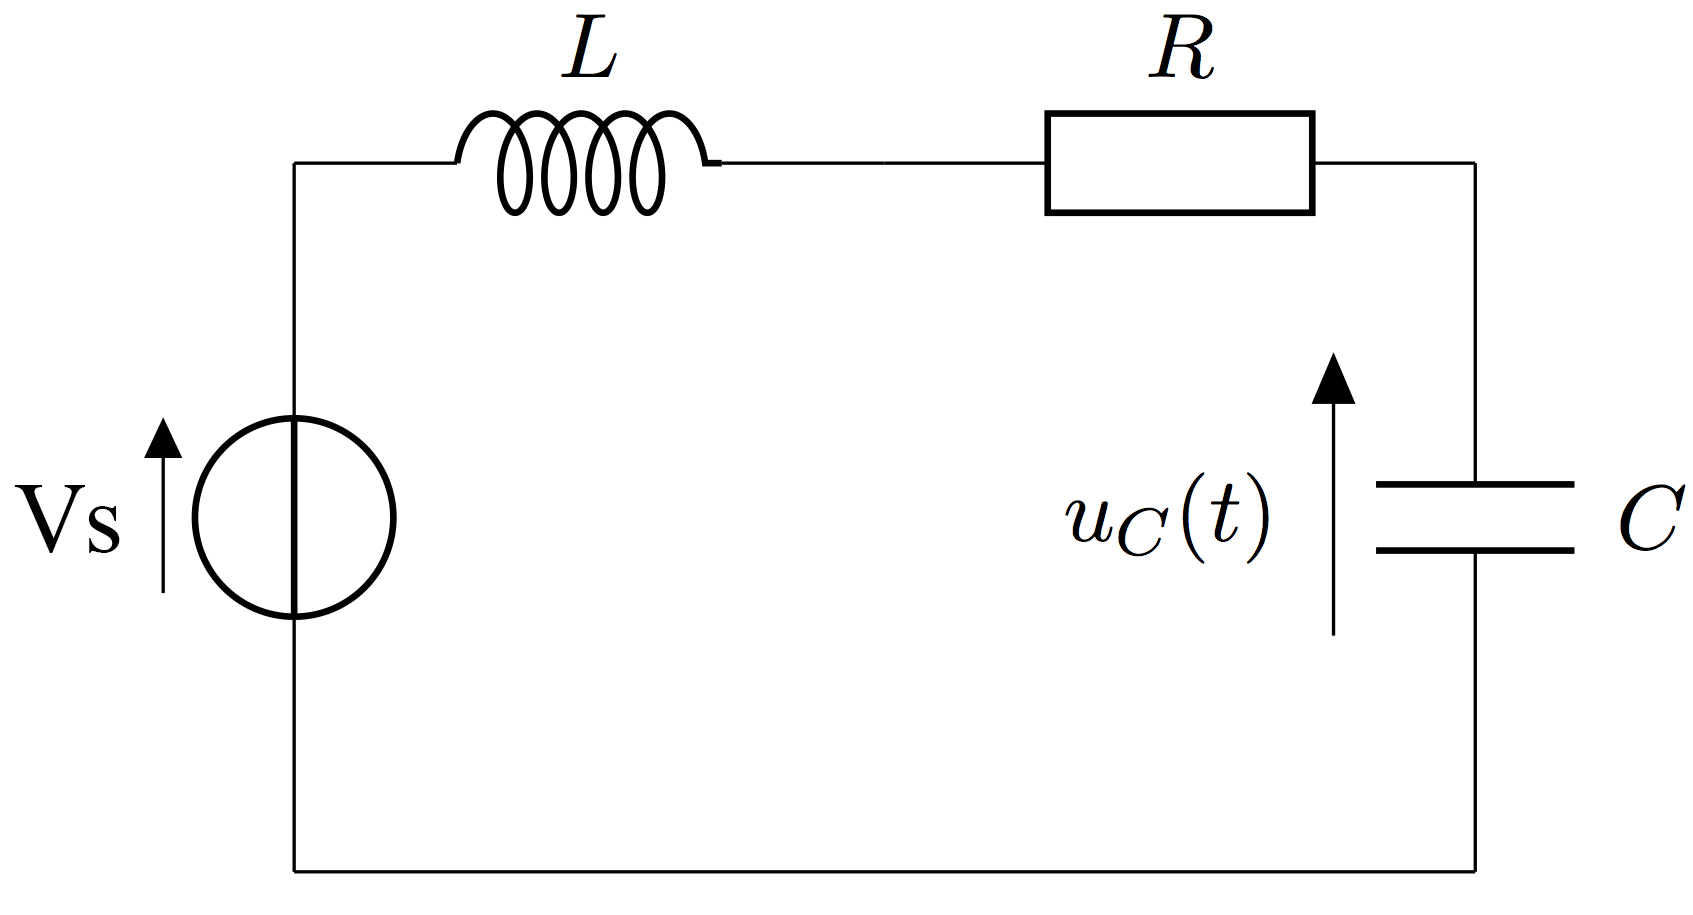
\includegraphics[scale=1]{fig1.jpg} 
\end{center}
Choix de R, L et C:

\begin{multicols}{2}
\setlength{\columnseprule}{0.4pt}
\begin{align*}
\text{on impose : }\\
\dfrac{\omega_p}{\omega_0}&=1,2\\
\omega_0 &= \dfrac{\omega_p}{1,2}\\
&=\dfrac{2\pi}{1,2.36.10^{-6}}\\
&\approx 1,5.10^5Hz\\
\end{align*}
\columnbreak
\begin{align*}
\omega_0 &= \dfrac{1}{\sqrt{L.C}} \\
\iff C&=\dfrac{1}{\omega_0^2.L}\\
&=3,1.10^{-9}F \\
(L&=15mH,\omega_0=1,5.10^5Hz)
\end{align*}
%\columnbreak\\
On veut également :
\begin{align*}
Q>5 &\implies \dfrac {1} {R}\sqrt {\dfrac {L} {C}}>5\\
&\implies \dfrac {1} {5}\sqrt {\dfrac {L} {C}}>R\\
&\implies R<\dfrac {1} {5}\sqrt {\dfrac {15.10^{-3}} {3.10^{-9}}}\\
&\implies R<440\Omega
\end{align*}
\end{multicols}
Après avoir ajouté ce nouvelle étage, on obtient une sortie sous forme d'enveloppe similaire à la modulation d'amplitude. Il suffit alors de placer un détecteur de crête (vu précédemment) et d'adapter sa constante de temps RC pour démoduler le signal.

\end{document}